%%%%%%%%%%%%%%%%%%%%%%%%%%%%%%%%%%%%%%%%%%%%%%%%%%%%%%%%%%%%%%%%%%%%%%%%%%%%%%%%%%%%%%%%%%%%%%%%%%%%%%%%%%%%%%%%%
%% Kapitel 2 - Stand der Forschung und Technik %%%%%%%%%%%%%%%%%%%%%%%%%%%%%%%%%%%%%%%%%%%%%%%%%%%%%%%%%%%%%%%%%%
%%%%%%%%%%%%%%%%%%%%%%%%%%%%%%%%%%%%%%%%%%%%%%%%%%%%%%%%%%%%%%%%%%%%%%%%%%%%%%%%%%%%%%%%%%%%%%%%%%%%%%%%%%%%%%%%%
\chapter{Stand der Forschung und Technik} \label{chap:stand}

Dieses Kapitel stellt die für diese Arbeit erforderlichen technischen und methodischen Grundlagen bereit. Zunächst werde in Abschnitt~\ref{sec:zuv} zentrale Begriffe und Konzepte der Zuverlässigkeitstechnik sowie das grundlegende statistische Verfahren zur Lebensdauer-Datenanalyse in Kombination mit Versuchsplänen erläutert.
Darauf aufbauend folgen in Abschnitt~\ref{sec:doe} die Einführung und die Einordnung von \acs{DoE} sowie der multivariaten Lebensdauermodellierung aus dem Stand der Technik und der Wissenschaft, die beide für die Entwicklung effizienter Lebensdauerversuchspläne maßgeblich sind.
Im Kontext der Lebensdauererprobung umfasst dies insbesondere typische, statistische Versuchspläne sowie Metriken und Indikatoren zur allgemeinen Bewertung der Versuchspläne.

\section{Zuverlässigkeitstechnik und Wahrscheinlichkeitstheorie} \label{sec:zuv}
Die Zuverlässigkeitstechnik befasst sich mit der probabilistischen Beschreibung der Lebensdauer technischer Produkte und Systeme.
Ziel ist die statistische Modellierung des Ausfallverhaltens unter Berücksichtigung der Funktionalität des Produkts bei relevanten Randbedingungen.
Eine zentrale Aufgabe besteht somit in der statistischen Charakterisierung des Ausfallbegriffs mithilfe deskriptiver Statistik sowie in der Parametrisierung geeigneter Verteilungen zur Abbildung des Lebensdauerverhaltens.
Die Modellierung kann - abhängig von den Randbedingungen - auf Basis \textit{einer einzelnen} Belastungsgröße oder \textit{mehrerer} Beanspruchungsparameter erfolgen, die gemeinsam den Produktausfall determinieren.
Ein grundlegendes Verständnis des Umgangs mit zufallsverteilten Lebensdauerereignissen ist daher eine elementare Voraussetzung für die statistische Versuchsplanung im Rahmen der Zuverlässigkeitstechnik.
Weiterführende Konzepte und vertiefte methodische Ansätze zur Zuverlässigkeitstechnik sowie zur statistischen Testplanung sind allen voran in der Standardliteratur von Bertsche und Dazer \cite{Bertsche.2022} dargelegt, an deren Vorgehensweise sich die nachfolgenden Ausführungen orientieren.

\subsection{Begriffe und Definitionen} \label{subsec:begriffezuv}
Der \textbf{Ausfall} eines technischen Produkts bezeichnet den Zeitpunkt innerhalb seiner Lebensdauer, zu dem die geforderte Funktionalität unter definierten Umgebungs- und Randbedingungen nicht mehr erfüllt ist - also das Lebensdauerende - engl. \textbf{\ac{EoL}}.
Als \textbf{Belastung} werden die von außen auf ein Produkt einwirkenden Einflussparameter - Kräfte und Momente im mechanischen Kontext - bezeichnet.
\textit{Einzelne} oder zeitgleich \textit{mehrere} Einflussparameter induzieren infolge der Produktgestalt daraus \textbf{Beanspruchungen}: innere Kräfte, Momente und lokale Spannungen.
Belastung und Beanspruchung sind die maßgeblichen Faktoren, welche die Lebensdauer determinieren.
Die \textbf{Ausfallzeit}, welche diese Zustandsänderung zeitlich definiert, wird im Allgemeinen als kontinuierliche Zufallsvariable $\sym{tau}>0$ aufgefasst.
So ergibt sich die Wahrscheinlichkeit, dass ein Produkt im Zeitraum bis $\sym{t}$ einen Funktionsverlust erleidet, zu
\begin{equation} \label{eq:probdef}
    \sym{F}(\sym{t})=\sym{Pr}(\sym{tau}\leq \sym{t}) = \int_{-\infty}^{\sym{t}} \sym{f}(\sym{t}) \,d\sym{t}.
\end{equation}
Diese Funktion beschreibt die \textbf{Ausfallwahrscheinlichkeit} - engl. \textbf{\ac{cdf}} - $\sym{F}(\sym{t})$, während die \textbf{Zuverlässigkeit}
\begin{equation} \label{eq:reldef}
    \sym{R}(\sym{t})=\sym{Pr}(\sym{tau} > \sym{t}) = 1 - \sym{F}(\sym{t}) = \int_{\sym{t}}^{\infty} \sym{f}(\sym{t}) \,d\sym{t} , \quad \sym{t} \geq 0.
\end{equation}
komplementär diejenige Wahrscheinlichkeit $\sym{R}(\sym{t}): \sym{RR}_{\geq 0} \rightarrow [0,1] \subset \sym{RR}$ quantifiziert, zu der das nicht reparierbare Produkt die realisierte Zeit $\sym{t}$ überlebt: also frei von Funktionsverlust bleibt und funktionsfähig ist \cite{Bertsche.2022,Birolini.2017,Meeker.2022,Yang.2007}.
Damit ist die Zuverlässigkeit mathematisch als reellwertige, monoton fallende und stetige Funktion definiert.
Gleichwohl ist $\sym{R}(\sym{t})$ keine universelle Eigenschaft, sondern damit vielmehr eine Funktion der Betriebsbedingungen.
Diese Bedingungen umfassen unter anderem eine oder mehrere Belastungsarten und deren Niveaus, Nutzungsverhalten sowie
spezifische Betriebsprofile. Mechanische, elektrische und thermische Belastungen treten dabei am häufigsten auf.

Die \textbf{Wahrscheinlichkeitsdichtefunktion} - engl. \textbf{\ac{pdf}} - $\sym{f}(\sym{t})$ der Ausfallzeit beschreibt, wie sich die Wahrscheinlichkeiten der Ausfälle über der Zeit verteilen.
Sie folgt somit der Ableitung der \ac{cdf}:
\begin{equation} \label{eq:pdfdef}
    \sym{f}(\sym{t}) = \frac{d}{d\sym{t}}\sym{F}(\sym{t}) = \frac{d}{d\sym{t}}\sym{Pr}(\sym{tau} \leq \sym{t}), \quad \sym{t} \geq 0.
\end{equation}
Damit repräsentiert $\sym{f}(\sym{t})$ die Ausfallintensität pro Zeiteinheit und ist proportional zur lokalen Änderungsrate der Ausfallwahrscheinlichkeit.
Als vierte fundamentale Größe der Zuverlässigkeitsanalyse wird außerdem die \textbf{Ausfallrate} (auch Hazard-Funktion) $\sym{lambda}(\sym{t})$ eingeführt.
Sie quantifiziert das momentane Ausfallrisiko eines Produkts zum Zeitpunkt $\sym{t}$, bedingt dadurch, dass es bis zu diesem Zeitpunkt überlebt hat ($\sym{R}(\sym{t}) > 0$).
Mathematisch ist sie als das Verhältnis der \ac{pdf} zur Zuverlässigkeitsfunktion $\sym{R}(\sym{t})$ definiert:
\begin{equation} \label{eq:hazarddef}
    \sym{lambda}(\sym{t}) = \lim_{\Delta \sym{t} \to 0} \frac{\sym{Pr}(\sym{t} < \sym{tau} \leq \sym{t} + \Delta \sym{t} | \sym{tau} > \sym{t})}{\Delta \sym{t}} = \frac{1}{\sym{R}(\sym{t})} \left[ - \frac{d\sym{R}(\sym{t})}{d\sym{t}} \right] = \frac{\sym{f}(\sym{t})}{\sym{R}(\sym{t})} .
\end{equation}
Die Ausfallrate $\sym{lambda}(\sym{t})$ ist von zentraler Bedeutung, da ihr zeitlicher Verlauf (z.B. konstant, steigend, fallend) direkte Rückschlüsse auf zugrundeliegende Ausfallmechanismen wie Frühausfälle, Zufallsausfälle oder
Verschleiß (vgl. "Badewannenkurve") zulässt \cite{Bertsche.2022,Yang.2007}.

\subsection{Deskriptive Statistik für Lebensdauerdaten} \label{subsec:stat}
Die im vorherigen Abschnitt definierten Funktionen $\sym{F}(\sym{t})$, $\sym{R}(\sym{t})$, $\sym{f}(\sym{t})$ und $\sym{lambda}(\sym{t})$ beschreiben das stochastische Ausfallverhalten eines Produktes auf einer theoretischen Populationsebene.
Für die praktische Anwendung im Engineering müssen diese Funktionen, respektive die Parameter der ihnen zugrundeliegenden Verteilungsmodelle, auf Basis von empirisch ermittelten Lebensdauerdaten jedoch approximiert werden.

Die deskriptive Statistik stellt die notwendigen Methoden zur initialen Charakterisierung, Quantifizierung und Aufbereitung dieser Stichprobendaten bereit.
Zur Beschreibung der Lebensdauerverteilungen sind \textbf{Lageparameter} und \textbf{Streuungsmaße} notwendig, die zunächst theoretisch (für die Grundgesamtheit) definiert und anschließend aus der Stichprobe berechnet werden.

Der primäre Lageparameter ist der \textbf{Erwartungswert} $\sym{mu}$ der Zufallsvariable $\sym{tau}$.
Er repräsentiert den Schwerpunkt von $\sym{f}(\sym{t})$ und wird für kontinuierliche Lebensdauerdaten berechnet als:
\begin{equation} \label{eq:theo_mean}
    \sym{mu} = \sym{E}[\sym{tau}] = \int_{0}^{\infty} \sym{t} \cdot \sym{f}(\sym{t}) d\sym{t}.
\end{equation}
Ein weiterer Lageparameter ist das \textbf{Quantil} $\symsub{t}{q}$ der Lebensdauer.
Es definiert den Zeitpunkt, zu dem $\sym{F}(\sym{t})$ den Anteil $\sym{q}$ (respektive das \textbf{Perzentil} in Prozentpunkten) erreicht:
\begin{equation} \label{eq:quantildef}
    \sym{F}(\symsub{t}{q}) = \sym{q}, \quad \sym{q} \in [0,1].
\end{equation}
Damit gibt das $\sym{q}$~-~Quantil denjenigen Lebensdauerwert an, unterhalb dessen der Anteil $\sym{q}$ aller betrachteten Produkte ausgefallen ist.
Ein spezieller Fall ist der \textbf{Median} $\sym{t}_{0.5}$, bei dem die Ausfallwahrscheinlichkeit 50\% beträgt:
\begin{equation} \label{eq:mediandef}
    \sym{F}(\sym{t}_{0.5}) = 0.5.
\end{equation}
Der Median beschreibt somit den Zeitpunkt, zu dem die Hälfte aller Produkte ausgefallen ist.

Das primäre Streuungsmaß ist die \textbf{theoretische Varianz} $\sym{sigma_sq}$, welche die mittlere quadratische Abweichung vom Erwartungswert beschreibt:
\begin{equation} \label{eq:theo_variance}
    \sym{sigma_sq} = \text{Var}[\sym{tau}] = \sym{E}[(\sym{tau} - \sym{mu})^2] = \int_{0}^{\infty} (\sym{t} - \sym{mu})^2 \cdot \sym{f}(\sym{t}) d\sym{t}.
\end{equation}
Da als theoretische Parameter üblicherweise unbekannt, werden $\sym{mu}$ und $\sym{sigma_sq}$ durch empirische Statistiken approximiert, die aus einer Stichprobe vom Umfang $\sym{n}$ (bestehend aus den Messwerten $\sym{x}_{1}, \dots, \symsub{x}{n}$) berechnet werden.
Diese werden wiederum als Realisierungen der Zufallsvariable $\sym{tau}$ aufgefasst.

Das gängige empirische Äquivalent für den Erwartungswert $\sym{mu}$ ist der \textbf{arithmetische Mittelwert} $\sym{x_bar}$:
\begin{equation} \label{eq:emp_mean}
    \sym{x_bar} = \frac{1}{\sym{n}} \sum_{\sym{i}=1}^{\sym{n}} \symsub{x}{i}.
\end{equation}
Analog wird die theoretische Varianz $\sym{sigma_sq}$ durch die \textbf{empirische Varianz} $\sym{s_sq}$ (eine erwartungstreue Kenngröße) approximiert:
\begin{equation} \label{eq:emp_variance}
    \sym{s_sq} = \frac{1}{\sym{n}-1} \sum_{\sym{i}=1}^{\sym{n}} (\symsub{x}{i} - \sym{x_bar})^2.
\end{equation}
Die \textbf{empirische Standardabweichung} $\sym{s} = \sqrt{\sym{s_sq}}$ dient entsprechend als Näherung für die theoretische Standardabweichung $\sqrt{\sym{sigma_sq}}$.\

Während die deskriptiven Statistiken $\sym{x_bar}$ und $\sym{s_sq}$ die zentrale Tendenz und die Streuung der vorliegenden Stichprobe quantifizieren, erlauben sie keine Extrapolation oder die Modellierung der zugrundeliegenden Funktionen $\sym{F}(\sym{t})$ und $\sym{f}(\sym{t})$ der Grundgesamtheit.
Um eine prädiktive, mathematische Beschreibung des stochastischen Ausfallverhaltens zu erhalten, müssen die in Abschnitt~\ref{subsec:begriffezuv} definierten Lebensdauerfunktionen durch geeignete parametrische Verteilungsmodelle approximiert werden.
Diese Verteilungsmodelle bieten eine geschlossene mathematische Form für \ac{cdf} und \ac{pdf} und ermöglichen es, das komplexe Ausfallverhalten durch eine geringe Anzahl von Parametern zu charakterisieren.\

In der Zuverlässigkeitstechnik hat sich hierfür die \textbf{Weibull-Verteilung} aufgrund ihrer hohen Flexibilität als das am häufigsten verwendete Modell etabliert.
Sie ist in der Lage, alle drei Phasen der "Badewannenkurve" (Frühausfälle, Zufallsausfälle, Verschleißausfälle) durch die Wahl ihrer Parametrisierung abzubilden.
Nichtsdestotrotz seien jedoch in Abhängigkeit des zugrundeliegenden physikalischen Ausfallmechanismus auch andere statistische Verteilungen, wie beispielsweise die Lognormal-Verteilung (häufig bei Ermüdungs-, Korrosions- oder Diffusionsprozessen) oder die Exponentialverteilung (zur Modellierung von Zufallsausfällen ohne Alterungseffekte), bezüglich der Anwendung in der Lebensdaueranalyse erwähnt.
Für weitere Ausführungen dazu sei an dieser Stelle jedoch auf bereits ausreichend diskutierte Werke \cite{Bertsche.2022,Yang.2007,Birolini.2017} verwiesen.

Die (zwei-parametrige) Weibull-Verteilung ist das Standardmodell zur Beschreibung der Lebensdauer von technischen Produkten \cite{Bertsche.2022}.
Sie wird durch den \textbf{Formparameter}  $\sym{b} > 0$ (Weibull-Modul) und die \textbf{charakteristische Lebensdauer} $\sym{T} > 0$ (Skalen- oder Lageparameter), welche dem 63,2-ten Perzentil $\sym{t}_{0,632}$ entspricht, beschrieben.
Folgt die Lebensdauer-Zufallsvariable $\sym{tau}$ dieser Verteilung, wird dies mathematisch als $\sym{tau} \sim \sym{W}(\sym{T}, \sym{b})$ notiert.
Die Einheit des Skalenparameter entspricht der Einheit des Messwertes ($\sym{t}$ in Stunden, Überrollungen, Kilometer, etc.).
Die (\ac{pdf}) der Weibull-Verteilung ist definiert als:
\begin{equation} \label{eq:weibull_pdf}
    \sym{f}(\sym{t}) = \frac{\sym{b}}{\sym{T}^{\sym{b}}} \sym{t}^{\sym{b}-1} \exp\left[ - \left(\frac{\sym{t}}{\sym{T}}\right)^{\sym{b}} \right], \quad \sym{t} > 0.
\end{equation}
Die (\ac{cdf}) ergibt sich durch Integration der \ac{pdf} zu:
\begin{equation} \label{eq:weibull_cdf}
    \sym{F}(\sym{t}) = 1 - \exp\left[ - \left(\frac{\sym{t}}{\sym{T}}\right)^{\sym{b}} \right], \quad \sym{t} > 0.
\end{equation}
Aus $\sym{f}(\sym{t})$ und $\sym{R}(\sym{t}) = 1 - \sym{F}(\sym{t})$ leitet sich die \textbf{Ausfallrate} $\sym{lambda}(\sym{t})$ der Weibull-Verteilung ab:
\begin{equation} \label{eq:weibull_hazard}
    \sym{lambda}(\sym{t}) = \frac{\sym{b}}{\sym{T}} \left(\frac{\sym{t}}{\sym{T}}\right)^{\sym{b}-1}, \quad \sym{t} > 0.
\end{equation}
Der Erwartungswert $\sym{mu}$ (vgl. Gl.~\eqref{eq:theo_mean}) und die Varianz $\sym{sigma_sq}$ (vgl. Gl.~\eqref{eq:theo_variance}) der Weibull-Verteilung lassen sich ebenfalls in geschlossener Form ausdrücken. Sie sind von der \textbf{Gamma-Funktion} $\sym{Gamma}(\cdot)$ abhängig, welche für $x > 0$ definiert ist als:
\begin{equation} \label{eq:gamma_func}
    \sym{Gamma}(x) = \int_{0}^{\infty} \sym{z}^{x-1} \exp(-\sym{z}) \,d\sym{z}.
\end{equation}
Der Erwartungswert $\sym{mu}$ der Weibull-verteilten Lebensdauer $\sym{tau}$ ergibt sich zu:
\begin{equation} \label{eq:weibull_mean}
    \sym{mu} = \sym{E}[\sym{tau}] = \sym{T} \cdot \sym{Gamma}\left(1 + \frac{1}{\sym{b}}\right).
\end{equation}
Die Varianz $\sym{sigma_sq}$ ist gegeben durch:
\begin{equation} \label{eq:weibull_variance}
    \sym{sigma_sq} = \sym{Var}[\sym{tau}] = \sym{T}^2 \left[ \sym{Gamma}\left(1 + \frac{2}{\sym{b}}\right) - \sym{Gamma}^2\left(1 + \frac{1}{\sym{b}}\right) \right].
\end{equation}
Die Ausprägung der erwähnten Flexibilität der Weibull-Verteilung ist durch \colorbox{yellow}{Abb. 2} nachvollziehbar.


\begin{figure}[h!]
    \centering
    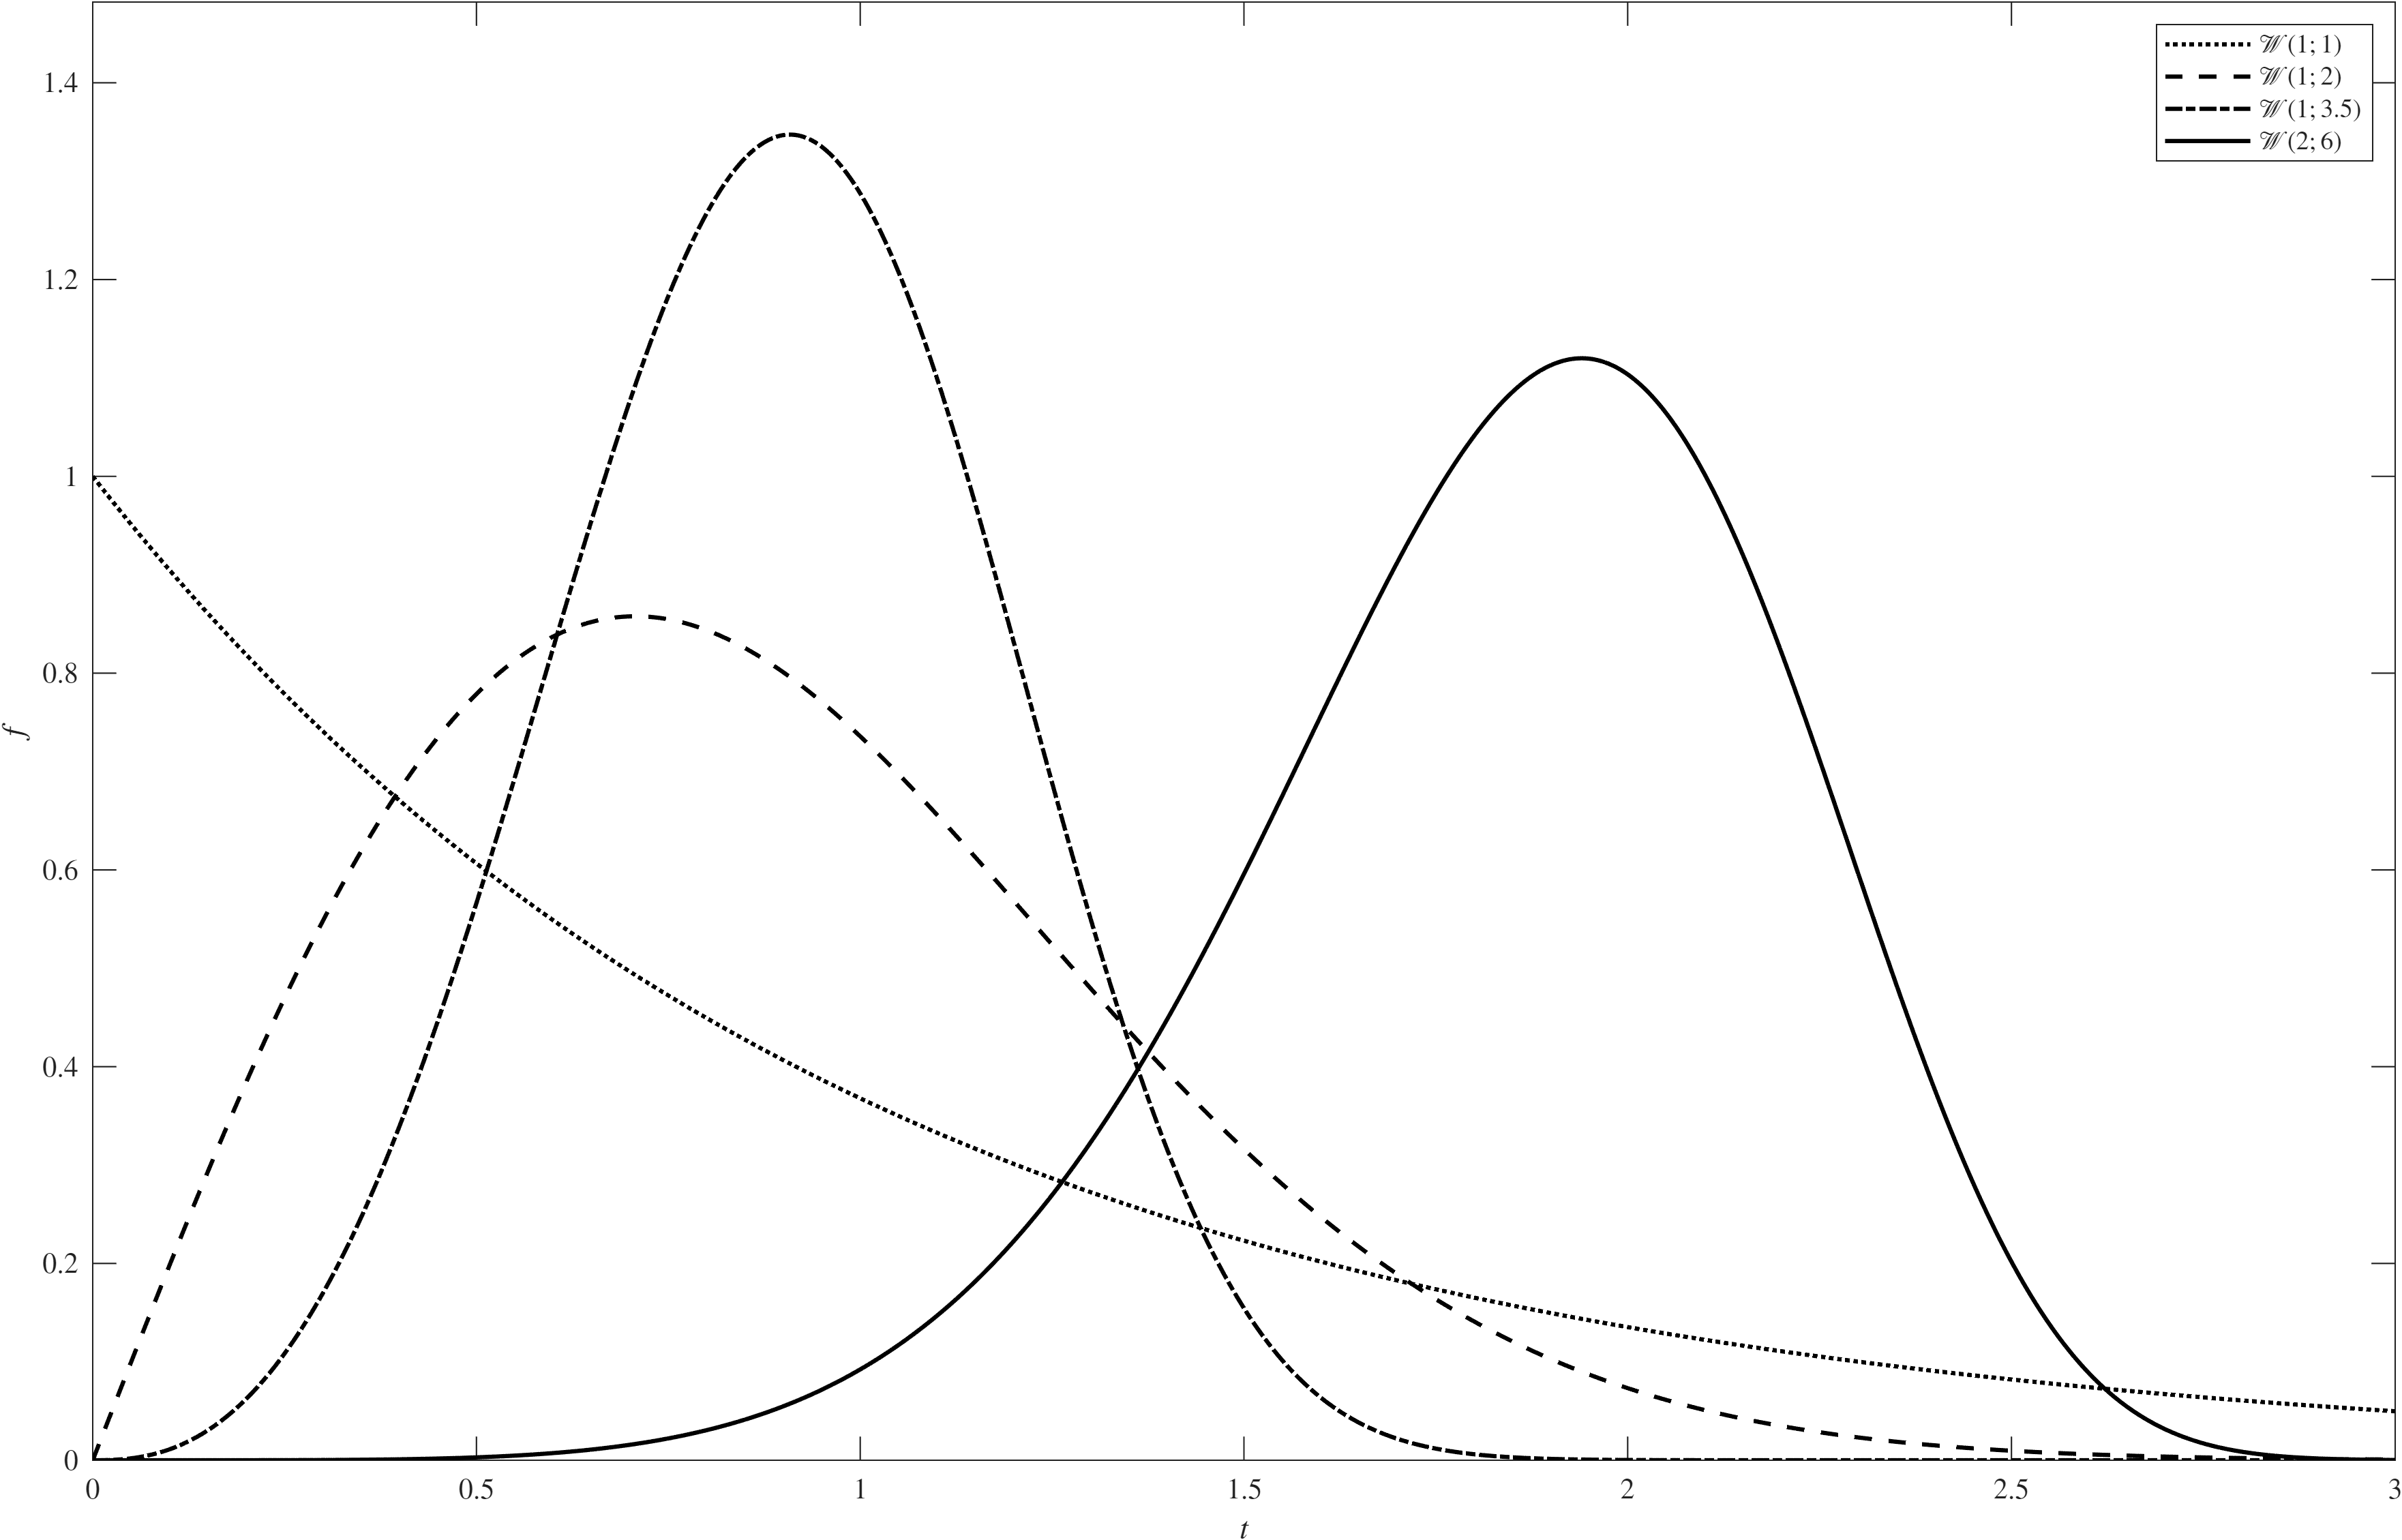
\includegraphics[width=0.8\textwidth]{plots/weibull_pdf_flexibility}
    \caption{Die Flexibilität der Weibull-Verteilung (als PDF eingebunden).}
    \label{fig:weibull_pdf}
\end{figure}
\subsection{Parameterschätzverfahren} \label{subsec:schätzer}

\section{Statistische Versuchsplanung und Modellbildung} \label{sec:doe}

\subsection{Grundbegriffe der statistischen Versuchsplanung} \label{subsec:begriffedoe}

\subsection{Statistische Lebensdauer-Versuchspläne} \label{subsec:pläne}

\subsection{Statistische Modellbildung} \label{subsec:model}
